\chapter{Diffusion}

\newpage

\section{Petits et gros mammifères $\bullet\bullet\circ\circ$}

Les mammifères sont des animaux à sang chaud, dont la chaleur est produite par le fonctionnement du métabolisme, qui dégage une puissance thermique $p_{th}$ par unité de volume. Cette puissance et la circulation sanguine permettent de maintenir une température $T_1$ à peu près uniforme et constante à l'intérieur du corps. Pour se prémunir contre les variations de température extérieur, les mammifères peuvent avoir une couche d'isolant (fourrure ou graisse) autour de leur corps. On souhaite connaitre la variation de cette épaisseur en fonction de la taille des mammifères. 

Pour simplifier, on considère que les mammifères sont des animaux sphériques de rayon $R$ recouverts d'une couche d'isolant d'épaisseur $e$ de capacité calorifique $c$, de masse volumique $\rho$ et de conductivité thermique $\lambda$. On notera $T(r)$ et $\vec{j}(r)$ le champ de température et le vecteur densité volumique de puissance en coordonnées sphériques, $r$ étant le rayon par rapport au centre de l'animal.

\begin{enumerate}

	\item La température extérieure étant $T_{0}$ et celle dans le mammifère étant maintenue dans tout son métabolisme à $T_1$, écrire les deux conditions aux limites vérifiées par la témpérature.
	
	\item En faisant un bilan d'énergie entre deux sphères concentriques de rayon $r$ et $r+dr$ situées dans la couche d'isolant, montrer la relation suivante :
	\begin{align*}
		\frac{1}{r^2}\frac{\partial }{\partial r}\left( r^2j_r\right) =-\rho c\frac{\partial T}{\partial t}
	\end{align*}
	
	\item Après avoir rappelé la loi de Fourier, montrer alors que la température vérifie, dans la couche d'isolant, la relation suivante :
	\begin{align*}
		\frac{\partial T}{\partial t}=\frac{\lambda}{\rho c_p r^2}\frac{\partial }{\partial r}\left( r^2\frac{\partial T}{\partial r}\right) 	
	\end{align*}
	Comment s'appelle cette équation ?

	\item On se place en régime permament. Résoudre cette équation avec les conditions aux limites.
	
	\item On introduit $\Phi=4\pi r^2j_r(r)$. Que représente cette quantité ? Dépend-elle de $r$ ? Montrer que $\Phi=4/3\pi R^3p_{th}$. En déduire :
	\begin{align*}
		\frac{R^2p_{th}}{3}=\frac{\lambda (R+e)}{e}(T_1-T_0)
	\end{align*}
	
	\item En déduire une expression du rapport de l'épaisseur de fourrure sur la taille de l'animal $e/R$. Pourquoi les gros mammifères résistent-ils mieux au froid ?

\end{enumerate}

\newpage

\begin{correction}

\begin{enumerate}

	\item On a simplement $T_{0}=T(R)$ et $T_1=T(R+e)$.
	
	\item On effectue un bilan d'enthalpie entre $r$ et $r+dr$ :
	\begin{align*}
		& r^2dr4\pi\times \mu c_p\times[T(r,t+dt)-T(r,t)]= \\
		& r^24\pi\times j(r,t)dt-(r+dr)^24\pi\times j(r+dr,t)dt
	\end{align*}
	On a donc :
	\begin{align*}
		 r^2 \mu c_p\times\frac{\partial T}{\partial t}(r,t)= \frac{\partial}{\partial r} \left( r^2j(r,t)\right)
	\end{align*}	
	Et alors, avec la loi de Fourier $j=-\lambda\frac{\partial T}{\partial r}$ :
	\begin{align*}
		\frac{\partial T}{\partial t}=\frac{\lambda}{\mu c_pr^2}\frac{\partial }{\partial r}\left( r^2\frac{\partial T}{\partial r}\right)
	\end{align*}

	\item La solution est $T(r)=A/r+B$. On trouve :
	\begin{align*}
		T(r) = \frac{R(R+e)}{re}(T_1-T_0)+\frac{R+e}{e}T_0-T_1\frac{R}{e}
	\end{align*}
	
	\item On introduit $\Phi=4\pi r^2j_r(r)$. Il s'agit du flux thermique (une puissance) à travers toute sphère de rayon $r$ autour du mamifère. Comme l'énergie se conserve, elle ne dépend pas de $r$ : $\Phi(r) =4\pi\times j(r)\times r^2=4\pi \lambda\frac{R(R+e)}{e}(T_1-T_0)$. La puisance dégagée par le mammifère est tout simplement $4/3\pi R^3p_{th}$, elle correspond à la puissance thermique passant par la sphère de rayon $R$, donc $\Phi =4/3\pi R^3p_{th}$. On trouve donc :
	\begin{align*}
		\frac{R^2p_{th}}{3}=\frac{\lambda (R+e)}{e}(T_1-T_0)
	\end{align*}
	
	\item On trouve :
	\begin{align*}
		\frac{e}{R}=\frac{1}{\frac{R^2p_{th}}{3\lambda(T_1-T_0)}-1}
	\end{align*}
	Ce rapport diminue d'autant plus que la taille de l'animal augmente.

\end{enumerate}

\end{correction}

\newpage

\section{Ailettes de refroidissement $\bullet\bullet\circ\circ$}

Certains moteurs à essence utilisent des ailettes métalliques pour évacuer leur chaleur avec l'air ambiant (on parle de refroidissement à air). Si ce système est beaucoup plus simple qu'un refroidissement liquide, la puissance de refroidissement est limitée et donc celle du moteur aussi.

On modélise cette ailette de refroidissement comme un cylindre d'axe $Ox$, de longueur $L$, de rayon $R$ constitué d'un matériau de conductivité $\lambda$, en contact avec l'air extérieur de température $T_e$. En $x=0$, l'ailette est en équilibre thermique avec le moteur à la température $T_0$. 

\begin{figure}[h!]
\centering
  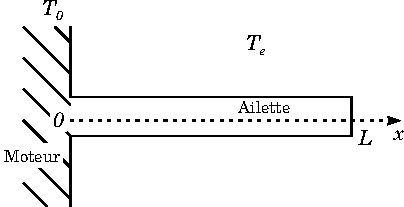
\includegraphics[width=0.7\textwidth]{diffusion_ailette.pdf}
\end{figure}

Pour une section de l'ailette de surface $\sigma$, à la température $T$, en contact avec l'air à $T_e$, évacue sa puissance thermique suivant la loi de Newton $P_s=h(T-T_e)\sigma$.

\begin{enumerate}

	\item En faisant un bilan d''énergie, déterminer en régime permanent l'équation différentielle vérifiée par la température $T(x)$.
	
	\item Donner l'expression de la température, si l'on suppose $L$ suffisament long (devant quoi ?)
	
	\item Déterminer la puissance thermique évacuée par l'ailette.
	
	\item Que devient cette étude si $L$ n'est pas suffisament grand ? Déterminer les nouvelles conditions aux limites.

\end{enumerate}

\newpage

\begin{correction}

\begin{enumerate}

	\item On trouve :
	\begin{align*}
		\frac{\partial^2 T}{\partial x^2} = \frac{2h}{\lambda R}(T(x)-T_e)
	\end{align*}
	
	\item On introduit $\delta=\sqrt{\lambda R/2h}$. Les solutions sont $T(x)=Ae^{x/\delta}+Be^{-x/\delta}+T_e$. Si $L\gg\delta$, alors $A=0$. On trouv nécessairement $B=T_0-T_e$.
	
	\item La puissance évacuée entre les tranches situées en $x$ et $x+dx$ est :
	\begin{align*}
		dP&=2\pi Rdx(T(x)-T_e) \\
		&=\pi Rdx(T_0-T_e)e^{-x/\delta}
	\end{align*}
	La puissance totale évacuée est donc :
	\begin{align*}
		P&=\int_0^L pi Rdx(T_0-T_e)e^{-x/\delta} \\
		&=\pi R\sqrt{2h\lambda R}(T_0-T_e)
	\end{align*}
	
	\item La condition à la limite $A=0$ n'est plus valide, on garde la solution générale. Il faut utiliser la continuité du flux thermique en $x=L$. On a alors :
	\begin{align*}
	& T_1=A+B+T_e \\
	& \Phi=-\lambda\pi R^2\frac{dT}{dx}(L)=h\pi R^2(T(L)-T_e)
	\end{align*}
Ces deux conditions réunies, on trouve (après calculs) :
\begin{align*}
	A=& \frac{(T_1-T_e)\left( 1-\frac{\lambda}{h\delta}\right) }{\left( 1-\frac{\lambda}{h\delta}\right) -\left( 1+\frac{\lambda}{h\delta}\right) e^{2L\delta}} \\
	B=&\frac{(T_1-T_e)\left( 1+\frac{\lambda}{h\delta}\right) }{\left( 1+\frac{\lambda}{h\delta}\right) -\left( 1-\frac{\lambda}{h\delta}\right) e^{-2L\delta}} 
\end{align*}

\end{enumerate}

\end{correction}

\newpage

\section{Lac gelé $\bullet\bullet\bullet\bullet$}

On s'intéresse à la glaciation d'un lac, et plus particulièrement de l'évolution au cours du temps de l'épaisseur de glace, notée $\xi(t)$, qui se forme à sa surface. L'interface entre l'atmosphère et la surface du lac se situe en $z=0$ et on considère qu'à $t=0$, le lac est encore libre de glace $\xi(t=0)=0$. On suppose que l'atmosphère est à la température constante $T_A=263$ K et que l'eau située sous la glace du lac est à la température de fusion $T_F$=273 K. 

\begin{figure}[h!]
\centering
  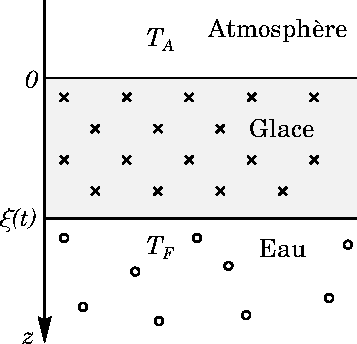
\includegraphics[width=0.4\textwidth]{diffusion_lac.pdf}
\end{figure}

Lors de la formation de la glace à l'interface $z=\xi(t)$, l'énergie thermique dégagée par la solidification de l'eau est évacuée à travers la glace jusqu'à l'atmosphère. On supposera que ce tranfert est instantané, ce qui revient à supposer que la glace a une capacité calorifique $c_g$ négligeable (hypothèse des régimes quasi-stationnaire).

D'autre part, les échanges thermiques entre l'atmosphère et la glace de la surface du lac sont modélisés par la loi de Newton : 
\begin{align*}
	\vec{j}_a=-h(T_0(t)-T_A)\vec{e}_z
\end{align*}
où $\vec{j}_a$ est la densité surfacique de flux thermique entre la glace et l'atmosphère, $T_0(t)$ est la température de la glace en $z=0$ et $h$ une constante égale à 42 W.m$^{-2}$.K$^{-1}$. Autrement dit, la surface du lac ne se thermalise pas instantanément avec l'atmosphère. 

On note par ailleurs $\rho_g=990$kg.m$^{-3}$ la masse volumique de la glace, $\lambda=2,1$ W.m$^{-1}$.K$^{-1}$ et la chaleur latente massique de fusion de l'eau $l_f=335$ kJ.kg$^{-1}$.

\begin{enumerate}

	\item Donner le profil de température $T(z,t)$ dans la glace en fonction de $T_0(t)$, $T_F$, $\xi(t)$ et $z$. 
	
	\item En déduire la température de surface $T_0(t)$ en fonction de l'épaisseur de glace $\xi(t)$, et $h$, $T_A$, $T_F$, $\lambda$.
	
	\item En faisant un bilan d'énergie sur le front de glaciation en $z=\xi(t)$, établir une relation entre $\xi(t)$ et $\dot{\xi}(t)$. En déduire l'équation différentielle suivante :
	\begin{align*}
		\left( 1+\frac{\xi(t)}{l_0}\right) \dot{\xi(t)}=v_0
	\end{align*}
	Préciser l'expression de $l_0$ et $v_0$.
	
	\item Donner une estimation numérique de $l_0$ et de $v_0$. En déduire un temps caractéristique $\tau_0$ dont on donnera aussi une estimation numérique. %L'approximation des régimes quasi-stationnaire est-elle valable ? 
	
	\item Déterminer l'évolution de $\xi(t)$ puis de $T_0(t)$ et donner l'allure de leur courbe. Combien de temps faut-il pour que 5 cm de glace ne se forment ?
	
\end{enumerate}	
	
\newpage

\begin{correction}

\begin{enumerate}

	\item En redémontrant l'équation de la chaleur, on trouverait :
	\begin{align*}
		\frac{\partial^2 T}{\partial z^2} = \frac{\rho c_g}{\lambda}\frac{\partial T}{\partial t} \simeq0
	\end{align*}
	car $c_g\simeq0$ dans le cadre de l'ARQS. On a alors :
	\begin{align*}
		T(z) = \frac{T_F-T_0(t)}{\xi(t)}z+T_0(t)
	\end{align*}
	
	\item Par conservation de l'énergie, la densité de flux thermique dans la glace $j_g(z,t)=-\lambda\frac{\partial T}{\partial z}$ est égale à la densité de flux thermique à l'interface $j_a$ donné par la loi de Newton :
	\begin{align*}
		& j_g(z=0,t)=j_a \\
		\Rightarrow & -\frac{\lambda}{\xi(t)}(T_F-T_0(t))=-h(T_A-T_0(t))
	\end{align*}
	On en déduit :
	\begin{align*}
		T_0(t)=\frac{T_F+\frac{h\xi(t)}{\lambda}T_A}{1+\frac{h\xi(t)}{\lambda}}
	\end{align*}
	
	\item On considère un volume d'eau $dV=S\times dz$ se transformant en glace durant un temps $dt$. Comme le front de galce avance à la vitesse $\dot{\xi}$, on a $dz=\dot{\xi}dt$. Ce volume dégage une énergie $dQ=l_f\rho_g\dot{\xi}dtS$ lors de sa transformation, qui est évacuée à travers le flux thermique dans la glace $dQ = -Sdt\times j_g(z=\xi,t)$. Le signe $-$ correspond au fait que l'énergie est évacuée vers l'atmosphère, donc selon $-\vec{e}_z$.
	
	On a alors : 
	\begin{align*}
		&\frac{\lambda}{\xi(t)}(T_F-T_0(t))=l_F\rho_g\dot{\xi}(t) \\
		\Rightarrow & T_F-\frac{T_F+\frac{h\xi(t)}{\lambda}T_A}{1+\frac{h\xi(t)}{\lambda}} =\frac{l_F\rho_g}{\lambda} \xi(t)\dot{\xi}(t) \\
		\Rightarrow & \frac{h}{l_F\rho_g}(T_F-T_A)=\left(1+\frac{h}{\lambda}\xi(t) \right) \dot{\xi}(t)
	\end{align*}
	
	On a donc :
	\begin{align*}
		\left( 1+\frac{\xi(t)}{l_0}\right) \dot{\xi(t)}=v_0
	\end{align*}
	Avec $l_0=\frac{\lambda}{h}$ et $v_0=\frac{h}{l_F\rho_g}(T_F-T_A)$. On peut vérifier l'homogénéité, qui est bien respectée. On remarque par ailleurs que $v_0=\dot{\xi}(t=0)$, qui correspond à la vitesse d'avancée du front de glace au début de la glaciation.
	
	\item $l_0= 0,05m$ et de $v_0=1,27\cdot10^{-6}$m/s. On définit un temps caractéristique $\tau_0$ comme tout simplement $\tau_0=l_0/V_0=39\cdot10^{3}$s.
	
	\item On intègre la relation précédente :
	\begin{align*}
			&v_0=\frac{l_0}{2}\frac{d}{dt}\left(1+\frac{\xi(t)}{l_0} \right)^2 \\
			\Rightarrow & \frac{2t}{\tau_0}=\left(1+\frac{\xi(t)}{l_0} \right)^2+C
	\end{align*}
	En tenant compte des conditions initiales, $\xi(0)=0$, on trouve $C=-1$.
	Donc, en résolvant l'équation du second degré et en prenant la racine positive, on obtient :
	\begin{align*}
		\xi(t) = l_0\left( \sqrt{1+\frac{2t}{\tau_0}}-1\right) 
	\end{align*}
	Et de même : 
	\begin{align*}
		T_0(t)=T_A+\frac{T_F-T_A}{\sqrt{1+\frac{2t}{\tau_0}}}
	\end{align*}
	
	Pour qu'il y ait 5 cm de glace, soit une épaisseur $\xi(t)=l_0$, il faut un temps $t=\frac{3}{2}\tau_0\simeq59\cdot10^{3}$s, soit environ 16h30. Cela montre bien que la vitesse de glaciation diminue, si elle se maintenait à $v_0$, il faudrait un temps $\tau_0$ pour geler ces 5cm, soit environ 11h. 

\end{enumerate}

\end{correction}

\newpage

\section{Transfert thermique et entropie $\bullet\bullet\circ\circ$}

On considère une barre métallique conductrice de section $S$, de longueur $L$, de résistivité électrique $\rho$ et de conductivité thermique $\lambda$. On suppose que ces extrémités sont maintenues aux températures $T_1$ et $T_2$ grâce à des thermostats, et que les parois extérieures sont calorifugées sur toute la longueur du barreau. En régime permanent, elle est parcourue par un courant $I$.

\begin{enumerate}

\item

\begin{enumerate}

	\item Justifier que  $p_{vol}=\rho I^2/S^2$

	\item Montrer que la température vérfie l'équation : 
		\begin{align*}
	  \lambda\frac{\partial^2 T}{\partial x^2} = - p_{vol}
	\end{align*}	
	Préciser l'expression de $p_{vol}$ en fonction des données de l'énoncé.

	\item Déterminer le profil de température $T(x)$ dans la barre, où $x$ est l'abcsisse le long de celui-ci.
	
	\item A quelle condition la température passe par un maximum ? 
	
	\item Calculer l'entropie $s_c$ créée par unité de temps et de volume dans la barre à une abscisse $x$. Commenter.
	
\end{enumerate}

\item On coupe désormais le courant dans la barre ($I=0$), puis une fois le nouveau régime permanent établi, on l'isole totalement des thermostats.

\begin{enumerate}
		
	\item Obtenir le nouveau profil de température juste avant que les deux thermostats soient retirés de la barre.
	
	\item Une fois les thermostats enlevés, quelle sera la température finale $T_\infty$ de la barre après avoir suffisament attendu ? En déduire la variation d'entropie de la barre.
	
\end{enumerate}

\end{enumerate}

\newpage

\section{Transfert thermique et entropie $\bullet\bullet\bullet\circ$}

On considère une barre métallique conductrice de section $S$, de longueur $L$, de résistivité électrique $\rho$ et de conductivité thermique $\lambda$. On suppose que ces extrémités sont maintenues aux températures $T_1$ et $T_2$ grâce à des thermostats, et que les parois extérieures sont calorifugées sur toute la longueur du barreau. En régime permanent, elle est parcourue par un courant $I$.

\begin{enumerate}

\item

\begin{enumerate}

	\item Déterminer le profil de température $T(x)$ dans la barre, où $x$ est l'abcsisse le long de celui-ci.
	
	\item A quelle condition la température passe par un maximum ? 
	
	\item Calculer l'entropie $s_c$ créée par unité de temps et de volume dans la barre à une abscisse $x$. Commenter.

\end{enumerate}

\item On coupe désormais le courant dans la barre ($I=0$), puis une fois le nouveau régime permanent établi, on l'isole totalement des thermostats.

\begin{enumerate}
		
	\item Obtenir le nouveau profil de température juste avant que les deux thermostats soient retirés de la barre.
	
	\item Une fois les thermostats enlevés, quelle sera la température finale $T_\infty$ de la barre après avoir suffisament attendu ? En déduire la variation d'entropie de la barre.
	
\end{enumerate}

\end{enumerate}

\newpage

\begin{correction}

\begin{enumerate}

\item

\begin{enumerate}

	\item Il faut d'abord obtenir l'équation de la chaleur lorsqu'une source de chaleur est présente dans le volume. L'équation de conservation (qui n'en est plus une !) devient :
	\begin{align*}
		c\rho\frac{\partial T}{\partial t} = -\frac{\partial j}{\partial x} + p_{vol}
	\end{align*}
	où $p_{vol} = \rho I^2/S^2$ est la puissance volumique dissipée par effet Joule. 
	L'équation de la chaleur devient donc :
	\begin{align*}
		\frac{\partial T}{\partial t} = \frac{\lambda}{c\rho}\frac{\partial^2 T}{\partial x^2} + \frac{p_{vol}}{c\rho}
	\end{align*}	
	En régime permanent :
	\begin{align*}
	  \lambda\frac{\partial^2 T}{\partial x^2} = - p_{vol}
	\end{align*}	
	En intégrant, on obtient :
	\begin{align*}
		T(x) = -\frac{p_{vol}x^2}{2\lambda}+Ax+B
	\end{align*}
	Avec les CL $T(0)=T_1$ et $T(L)=T_2$, on trouve :
	\begin{align*}
		T(x) = \frac{p_{vol}}{2\lambda}x(L-x)+\frac{T_2-T_1}{L}x+T_1
	\end{align*}
	\item Il y a plusieurs façon de répondre à la question. Je préfère utiliser la condition où $T'(L)=0$, cad que la puissance électrique chauffe suffisament pour tordre la courbe de température de sorte à ce que la dérivée deviennent nulle en $x=L$ (en considérant que $T_2>T_1$).
	Comme on a :
	\begin{align*}
		T'(x) = \frac{p_{vol}}{2\lambda}(L-2x)+\frac{T_2-T_1}{L}
	\end{align*}
	La condition $T'(L)=0$ donne alors : 
	\begin{align*}
		p_{vol} = 2\lambda\frac{T_2-T_1}{L^2}
	\end{align*}
	
	\item On effectue un bilan d'entropie sur le système constitué d'une tranche de barre entre $x$ et $x+dx$ du barreau durant un temps $dt$ :
	\begin{align*}
		dS = \delta s_e(x) - \delta s_e(x+dx) +\delta s_c
	\end{align*}
Il s'agit, pour l'entropie échangée, du même raisonnement que dans le cas d'une machine thermique avec deux sources extérieures, un échange d'netropie en $x$ et un autre en $x+dx$. $\delta s_c$ est l'entropie crée durant $dt$

En RP, $dS = 0$ et $\delta s_e(x)=\frac{\delta Q(x)}{T(x)}=Sdt\frac{j(x)}{T(x)}$. Alors :
\begin{align*}
	& Sdt\frac{j(x)}{T(x)} - Sdt\frac{j(x+dx)}{T(x+dx)} +\delta s_c = 0 \\
	& \delta s_c =  -S\lambda dt\left( \frac{1}{T(x+dx)}\frac{\partial T}{\partial x}(x+dx)\right) + S\lambda dt\left( \frac{1}{T(x)}\frac{\partial T}{\partial x}(x)\right) \\
	& \frac{ \delta s_c}{Sdxdt}=-\lambda\frac{\partial}{\partial x}\left(\frac{1}{T(x)}\frac{\partial T}{\partial x} \right) = -\frac{\lambda}{T(x)}\frac{\partial^2 T}{\partial x^2} + \frac{\lambda}{T^2(x)}\left( \frac{\partial T}{\partial x} \right) ^2
\end{align*}
L'entropie crée par unité de volum eet de temps est donc :
\begin{align*}
	\frac{s_{c,vol}}{dt}  = \frac{\rho I^2}{S^2 T}+ \frac{\lambda}{T^2(x)}\left( \frac{\partial T}{\partial x} \right) ^2 >0
\end{align*}
Le premier terme correspond à l'entropie crée par effet Joule, le second par les transferts thermiques.

\end{enumerate}

\item

\begin{enumerate}

	\item On peut réutiliser les résultats de la question précédente, pour $I=0$ :
		\begin{align*}
		T(x) = \frac{T_2-T_1}{L}x+T_1
	\end{align*}
	
	\item Il y a plusieurs façon de calculer la température finale. Pour ma part, j'utilise la conservation de l'énergie thermique $U$ de la barre lors de la transformation. Comme celle-ci est totalement isolée, on a :
	$U(t=0)=U_\infty=SL\mu c T_\infty$ où $\mu$ est la masse volumique de la barre.
	Or, l'énergie interne à $t=0$ est la somme de toutes les énergies internes du barreau d'épaisseurs $dx$ :
	\begin{align*}
		U(t=0) &= c\mu S\int_0^LdxT(x) \\
		&=c\mu SL\frac{T_1+T_2}{2}
	\end{align*}
	donc $T_\infty = \frac{T_1+T_2}{2}$, on trouve bien que la température finale correspond à la moyenne des empératures extrêmes. 
	Pour le calcul de l'entropie, on se base sur la variation d'entropie d'un solide lors d'une transformation d'une température à une autre. Plus précisément, un élément $Sdx$ de la barre à l'abscisse $x$ passe de la témprature $T(x)$ à $T_\infty$. Sa variation d'entropie est donc :
	\begin{align*}
		\Delta (\delta S) = \mu c S dx \ln\left(\frac{T_\infty}{T(x)} \right) 
	\end{align*}
	Donc pour l'ensemble de la barre :
	\begin{align*}
		\Delta S &= -\mu c S \int_0^Ldx \ln\left(\frac{T(x)}{T_\infty} \right) \\
		& = -\mu c S\frac{L}{T_2-T_1}\int_{T_1}^{T_2}dT\ln\left(\frac{T}{T_\infty}\right)
	\end{align*}
Finalement : 
\begin{align*}
\Delta S = Mc \left( 1 + \frac{T_1}{T_2-T_1}\ln\left(\frac{2T_1}{T_1+T_2}\right) - \frac{T_2}{T_2-T_1}\ln\left(\frac{2T_2}{T_1+T_2}\right)\right)
\end{align*}

\end{enumerate}

\end{enumerate}

\end{correction}

\newpage

\section{Combustion d'une poutre de bois $\bullet\bullet\bullet\circ$}

On considère une poutre en bois homogène de section carrée $S$ et de longueur $L$ rentrant en combustion à l'instant $t=0$ en $x=0$. On cherche à comprendre la progression de la combustion le long de la poutre, en supposant que celle-ci est uniquement dûe à la diffusion de la chaleur dans le bois. 
A l'instant $t$, on distingue la combustion en 3 zones distinctes :
\begin{itemize}
	\item[-] une zone brulée, située entre $x=0$ et $x_1(t)$, à la température uniforme $T_c=720$ K dite de combustion ;
	\item[-] une zone dans laquelle s'effectue la combustion, située entre $x_1(t)$ et $x_2(t)$, dégageant une puissance thermique massique $P_c=4,0\times10^3$ W.kg$^{-1}$ ;
	\item[-] et une zone inaltérée, où le bois est encore intact, située entre $x_2(t)$ et $L$
\end{itemize}
La température $T(x,t)$ dans la zone en combustion et celle de la zone inaltérée augmentent par diffusion au cours du temps jusqu’à atteindre les températures de combustion $T_c$ et d’inflammation du bois $T_i=$520 K, conduisant à l’avancement des frontières $x_1(t)$ et $x_2(t)$ au cours du temps. Ainsi, tant que la poutre n’a pas fini de bruler, on a toujours $T(x_1(t),t)=T_c$ et $T(x_2(t),t)=T_i$. D'autre part, loin du front de combustion $x_1(t)$, la température de la poutre est $T_\infty=320$ K.

\begin{figure}[h!]
\centering
  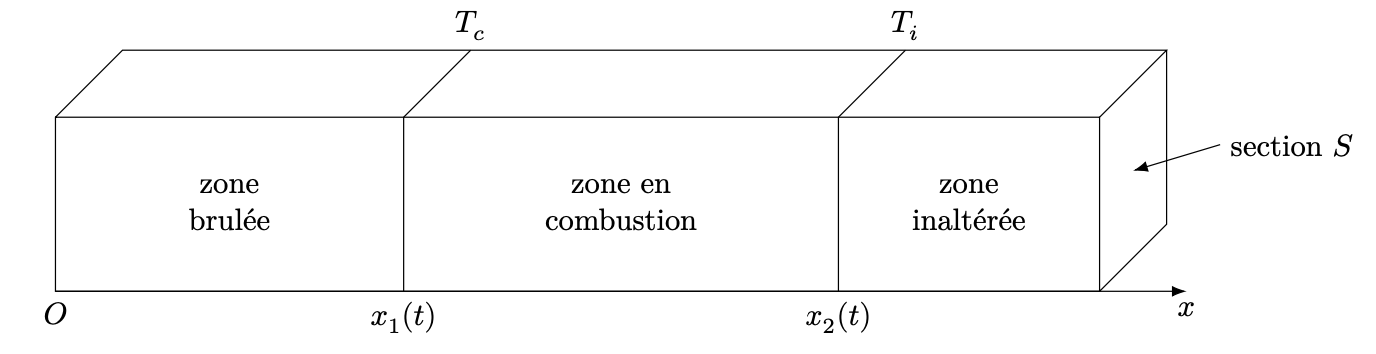
\includegraphics[width=0.9\textwidth]{poutre.png}
\end{figure}

On considère enfin que le bois brulé, en combustion ou inaltéré est un même matériau homogène, de capacité calorfique massique à pression constante $c_p=2,0\times10^3$ J.K$^{-1}$.kg$^{-1}$, de diffusivité thermique $D=1,0\times10^{-7}$m$^2$.s$^{-1}$ et de masse volumique $\mu=850$kg.m$^{-3}$.

\begin{enumerate}

\item

\begin{enumerate}

\item En effectuant un bilan d'enthalpie sur un élément de bois compris entre $x$ et $x+dx$ dans la zone en combustion, montrer que la température vérifie l'équation suivante :
	\begin{align*}
		\frac{\partial T}{\partial t}=D\frac{\partial^2 T}{\partial x^2} + \kappa
	\end{align*}
	Préciser l'expression de $\kappa$.
	\item De même, trouver l'équation vérifiée par $T$ dans la zone brulée et inaltérée. 

\end{enumerate}

\item On se propose de résoudre les équations précédentes sous forme d’une onde se propageant dans la poutre. On pose $u=x-ct$ où $c$ est une constante positive et on effectue le changement de variable $T(x,t)=\theta(u)$.

\begin{enumerate}

\item Que représente physiquement $c$ ? 
	\item Déterminer les équations différentielles régissant la fonction $\theta(u)$ dans les trois zones, puis montrer que les solutions peuvent s'écrire :
	\begin{align*}
		\left\{
    \begin{array}{ll}
        \theta(u)=a_1 & \mbox{pour } u<u_1 \\
       \theta(u)=a_2 + b_2\exp\left( -\frac{c}{D}u\right)  - \frac{\kappa}{c}u & \mbox{pour } u_1<u<u_2 \\
       \theta(u)=a_3 + b_3\exp\left( -\frac{c}{D}u\right)  u_2<u
    \end{array}
\right.
	\end{align*}
	\item Déterminer les expressions de $a_1$ et de $a_3$ avec les données de l'énoncé, puis expliciter les conditions permettant de trouver $a_2$, $b_2$ et $b_3$ (on ne cherchera pas à obtenir leur expression).
	\item Tracer l'allure de la courbe $\theta(u)$. Commenter. 

\end{enumerate}

\end{enumerate}

\newpage	

\section{Température dans une planète naine $\bullet\bullet\circ\circ$}

On s'intéresse au profil de température au sein d'une planête naine, faisant 100 km de rayon. On suppose qu'elle est intégralement constitué de roches proches du granit (conductivité thermique $\lambda = 3,5$ W.m$^{-1}$.K$^{-1}$, masse volumique $\mu=2700$ kg.m$^{-3}$ et capacité calorifique massique $c_p=790$ J.K$^{-1}$.s$^{-1}$), sans activité géologique, c'est-à-dire que l'astre est figé, sans convection possible à l'intérieur. Il existe de surcroit une activité radioactive dûe à la présence de thorium 232($^{232}$Th, masse molaire $M=232$ g.mol$^{-1}$) uniformément réparti dans le volume, dont la désintégration dégage une énergie $\varepsilon=5,6\times10^{-12}$ J, avec une demi-vie de $\tau=14\times10^{10}$ années.

\begin{enumerate}

\item

\begin{enumerate}

\item La concentration massique de thorium étant de l'ordre de 10 parties par million (ppm), estimer la puissance volumique $P_r$ due à la désintégration du thorium.
	
	\item Le problème étant supposé à symétrie sphérique, effectuer un bilan d'enthalpie entre deux couches adjacentes de roche de rayon $r$ et $r+dr$ et montrer que la température vérifie l'équation suivante :
	\begin{align*}
		\frac{\partial T}{\partial t}=\frac{D}{r^2}\frac{\partial }{\partial r}\left( r^2\frac{\partial T}{\partial r}\right)  + \kappa		
	\end{align*}
Préciser l'expression de $\kappa$ et de $D$.

	\item Montrer que l'on peut se placer dans le régime quasi stationnaire $T(r,t)\simeq T(r)$, c'est-à-dire que l'activité nucléaire varie très lentement par rapport au temps caractéristique $\tau_d$ de diffusion thermique. 
	
	\item Exprimer l'expression du champ de température $T(r)$ à l'aide de deux constantes d'intégration. Montrer que l'une d'entre elle est nécessairement nulle.

\end{enumerate}

\item La planète perd de l'énergie thermique par rayonnement, qui part dans l'espace depuis sa surface. La puissance thermique associée à ce rayonnement suit la loi de Stefan-Boltzmann $\phi=\sigma T_s^4$, où $\phi$ est la puissance rayonnée par unité de surface à la surface de la planète, $\sigma=5,67\times10^{-8}$ W.m$^{-2}$.K$^{-4}$ une constante et $T_s$ la température à la surface de l'astre.

\begin{enumerate}

	 \item En utilisant la loi de Stefan-Boltzmann, déterminer la seconde constante d'intégration et donner l'expression de la température $T(r)$.
	 
	 \item Donner la valeur de la température au centre de la planète et à la surface.

\end{enumerate}

\end{enumerate}

On donne, pour les coordonnées sphériques : $\vec{\mathrm{grad}} f\cdot \vec{e}_r = \frac{\partial f}{\partial r}$

\newpage

\begin{correction}

\begin{enumerate}

\item

\begin{enumerate}

	\item La concentration de thorium est de $c=10\times10^{-6}\times\mu$=27g.m$^{-3}$, soit une quantité $n=cN_A/M=7,00\times10^{22}$ atomes de thorium par m$^3$. La puissance peut être estimée par l'énergie $\varepsilon$ d'une désintégration divisée par le temps de demi-vie $\tau$ (ce qui correspond peu ou prou à l'activité nucléaire, un facteur $\ln2$ près), soit $P_r=\frac{\varepsilon n}{\tau}=8,90\times10^{-8}$ W.m$^{-3}$.
	
	\item On effectue un bilan d'enthalpie entre $r$ et $r+dr$ :
	\begin{align*}
		& r^2dr\sin\theta d\theta d\phi\times \mu c_p\times[T(r,t+dt)-T(r,t)]= \\
		& r^2\sin\theta d\theta d\phi\times j(r,t)dt-(r+dr)^2\sin\theta d\theta d\phi\times j(r+dr,t)dt + P_rdt r^2dr\sin\theta d\theta d\phi
	\end{align*}
	On a donc :
	\begin{align*}
		 r^2 \mu c_p\times\frac{\partial T}{\partial t}(r,t)= \frac{\partial}{\partial r} \left( r^2j(r,t)\right) + r^2\times P_r
	\end{align*}	
	Et alors, avec la loi de Fourier $j=-\lambda\frac{\partial T}{\partial r}$ :
	\begin{align*}
		\frac{\partial T}{\partial t}=\frac{D}{r^2}\frac{\partial }{\partial r}\left( r^2\frac{\partial T}{\partial r}\right)  + \kappa		
	\end{align*}
Avec $\kappa=P_r/(\mu c_p)$ et de $D=\lambda/(\mu c_p)$.

	\item Le temps caractéristique de diffusion thermique est estimé comme $\tau_d \simeq L^2/D=L^2\mu c_p/\lambda=6,09\times10^{15}$ s, soit 0,19 milliard d'années. C'est long mais toujours bien inférieur à 14 milliards d'années, qui est le temps caractéristique de décroissance radioactive du thorium. La planète a donc le temps d'être à tout instant thermalisée avec l'extérieur. 
	
	\item On peut donc estimer que le terme $\partial T/\partial t$ est nul. L'équation de diffusion devient :
	\begin{align*}
		\frac{D}{r^2}\frac{\partial }{\partial r}\left( r^2\frac{\partial T}{\partial r}\right) =  -\kappa		
	\end{align*}
	L'intégration fait apparaître deux constantes d'intégration, $A$ et $B$ :
	\begin{align*}
		T(r) = -\frac{\kappa}{6D}r^2-\frac{A}{r}+B
	\end{align*}
	La température étant définie en tout point de la planête, y compris en $r=0$, on a nécessairement $A=0$. 
	
\end{enumerate}

\item

\begin{enumerate}

	 \item La loi de Stefan-Boltzmann donne une seconde CL : $j(r=R)=-\lambda\frac{\partial T}{\partial r}(r=R)=\sigma T^4(r=R)$. On a donc :
	 \begin{align*}
	 	\lambda\frac{\kappa}{3D}R=\sigma\left(B-\frac{\kappa}{6D}R^2\right)^4
	 \end{align*}
	 et donc :
	 \begin{align*}
	 	B = \sqrt[4]{\frac{P_r R}{3\sigma}}+\frac{\kappa}{6D}R^2
	 \end{align*}
	 Finalement :
	 \begin{align*}
	 	T(r) = \frac{\kappa}{6D}\left( R^2 - r^2\right) +\sqrt[4]{\frac{P_r R}{3\sigma}}
	 \end{align*}
	 
	 \item Pour $T(0)=\sqrt[4]{\frac{P_r R}{3\sigma}}+\frac{\kappa}{6D}R^2\simeq63$ K et $T(R)=\sqrt[4]{\frac{P_r R}{3\sigma}}\simeq 20$ K.

\end{enumerate}	

\end{enumerate}

\end{correction}

\newpage

\section{Une tente au soleil $\bullet\bullet\bullet\bullet$}

Un campeur se trouve allongé dans sa tente canadienne. Le soleil se lève et éclaire une des faces de la tente, mais pas l'autre. Pour se refroidir, est-ce une bonne idée pour notre campeur de se mettre en position assise ? 
	
\vspace*{2cm}	
	
\begin{figure}[h!]
\centering
  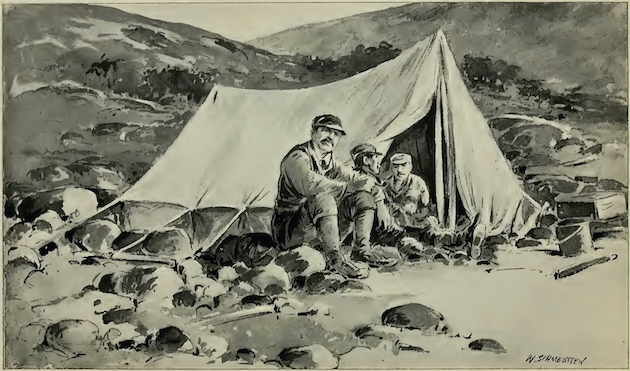
\includegraphics[width=0.7\textwidth]{tente.jpg}
\end{figure}

\newpage	

\section{Diffusion de particules dans un récipent en rotation $\bullet\bullet\bullet\circ$}

Des particules de masse $m$, de rayon $a$ et de masse volumique $\rho_p$ sont en suspension dans un solvant de masse volumique $\rho_s$ et de viscosité $\eta$, contenu dans un récipent. Elles subissent par ailleurs une force de frottement fluide $-6\pi\eta a\vec{v}$ lorsqu'elles sont en mouvement à la vitesse moyenne $\vec{v}$. Le coefficient de diffusion de ces particules dans le solvant est noté $D$.

\begin{enumerate}

\item

\begin{enumerate}

\item En régime permanent, établir la vitesse moyenne d'une particule isolée qui sédimente, soumise à son poids, à la poussée d'Archimède et à la force de frottement fluide.	On introduira la masse effective $m^*=m\left( 1-\frac{\rho_s}{\rho_p}\right) $. Quel est le flux de particules $\vec{j}_s$ associé à cette sédimentation ? 
	
	\item Ce flux de sédimentation est compensée par le phénomène de diffusion. Expliquer le phénomène. 
	
	\item En faisant un bilan de particules sur un volume élémentaire, montrer que la concentration de particule $c$ est reliée à $\vec{j}_s$ et au flux de particule $\vec{j}_D$ dû à la diffusion par la relation suivante :
	\begin{align*}
		\frac{\partial c}{\partial t}=-\diver(\vec{j}_D+\vec{j}_s)
	\end{align*}
	
	\item En déduire la concentration de particule $c(z)$ dans le récipient en régime permanent.

\end{enumerate}

\item On fait tourner désormais le récipient à une vitesse angulaire $\omega$, soumettant les particules à une force centrifuge $\vec{f}_r=m\omega^2r\vec{e}_r$. On néglige désormais le poids des particules.

\begin{enumerate}

	\item Montrer que la concentration en particules vérifient l'équation suivante :
	\begin{align*}
		\frac{\partial c}{\partial t}=\frac{1}{r}\frac{\partial }{\partial r}\left(r\left(D\frac{\partial c}{\partial r} -sr\omega^2c(r) \right) \right)
	\end{align*}
	Préciser l'expression de $s$.
	
	\item En déduire la concentration de particules en régime permanent. 

\end{enumerate}

\end{enumerate}

\newpage

\begin{correction}

\begin{enumerate}

\item

\begin{enumerate}
	
	\item La poussée d'Archimède est définie comme :
	\begin{align*}
		\vec{\pi}=\rho_s\frac{m}{\rho_p}g\vec{e}_z
	\end{align*}
	Elle est égale au poids du volume de solvant déplacé et est opposée à la gravitation. 
	Le bilan des forces devient en régime permanent, appléiqué sur une particule :
	\begin{align*}
		\vec{0} = \vec{\pi} -mg\vec{e}_z-6\pi\eta a\vec{v}
	\end{align*}
	La vitesse moyenne qui es résulte est donc :
	\begin{align*}
		\vec{v} = -\frac{mg}{6\pi\eta a}\left(1-\frac{\rho_s}{\rho_p} \right)\vec{e}_z=-\frac{m^*g}{6\pi\eta a}\vec{e}_z
	\end{align*}
	On trouve bien que la particule tombe (respectivement remonte) si sa masse volumique est supérieure à celle du solvant (respectivement inférieure).
	Le flux associé de particules est $\vec{j}_s=c\times\vec{v}$.
	
	\item Si on regardait le phénomène sans diffusion, toutes les particules tomberaient au fond du récipient et s'agglutineraient. Or, au fur et à mesure qu'elles tombent, leur concentration $c(z)$ augemente, générant un courant de diffusion $\vec{j}_D=-D\vec{\grad}(c)$ opposé qui fait "remonter" les particules. Un équilibre s'établit.
	
	\item On refait le bilan élémentaire du flux de particule sur un volume élémentaire, en ajoutant le courant $\vec{j}_s$. On trouve alors facilement :
	\begin{align*}
		\frac{\partial c}{\partial t}=-\diver(\vec{j}_D+\vec{j}_s)
	\end{align*}
	
	\item En régime permanent : 
	\begin{align*}
		\diver(\vec{j}_D+\vec{j}_s)=0
	\end{align*}
	Comme les flux ne sont que selon $\vec{e}_z$, en intégrant par rapport à $z$, on a $\vec{j}_D+\vec{j}_s=A$. En $z=0$, au fond du récipient, le flux total est nécessairement nul car les particules ne peuvent pas traverser le récipient. Donc :
	\begin{align*}
		\vec{j}_D+\vec{j}_s=0
	\end{align*}
	Et alors :
	\begin{align*}
		c(z)\frac{m^*g}{6\pi\eta a} &= -D\frac{\partial c}{\partial z} \\
		c(z) &+ L\frac{\partial c}{\partial z}=0
	\end{align*}
	avec $L=\frac{6\pi\eta aD}{m^*g}$.
	Et donc :
	\begin{align*}
		c(z)=c_0\exp\left[-\frac{z}{L} \right] 
	\end{align*}
	
\end{enumerate}

\item

\begin{enumerate}

	\item Même raisonnement que précédemment, en remplaçant la force du poids par la force centrifuge. Attention, il y a toujours une poussée d'Archimède ! On trouve que $\vec{v}=\frac{m^*\omega^2 r}{6\pi\eta a}\vec{e}_r$. Les particules sont bien ramenées vers l'extérieurs si elles sont plus denses que le solvant. Le courant de particules associé est $j_c=c(r)\vec{v}$, la concentration ne dépendant que de $r$ dans ce cas-là.
	
	On trouve ensuite, avec un bilan en coordonnées cylindriques :

	\begin{align*}
		\frac{\partial c}{\partial t}=\frac{1}{r}\frac{\partial }{\partial r}\left(r\left(D\frac{\partial c}{\partial r} -sr\omega^2c(r) \right) \right)
	\end{align*}
	avec $s=\frac{m^*}{6\pi\eta a}$. 
	
	\item Même raisonnement que précédemment, pour trouver que $D\frac{\partial c}{\partial r} -sr\omega^2c(r)=0$.
	On trouve alors que :
	\begin{align*}
	 \frac{\partial c}{\partial r}=\frac{r}{L^2}c(r)
	\end{align*}
	avec $L=\sqrt{s\omega^2/D}$.
	La solution est :
	\begin{align*}
		c(r)=c_0\exp\left[\frac{r^2}{2L^2} \right] 
	\end{align*}

\end{enumerate}

\end{enumerate}

\end{correction}


\newpage

\section{Diffusion à contre-courant $\bullet\bullet\bullet\circ$}

Dans un tuyau de section $S$ circule un solvant à la vitesse $-v_0\vec{e}_x$, où $x$ est l'axe le long du tuyau. En $x=0$, on injecte à travers une petite ouverture un colorant dans le tuyau, avec un débit molaire $n^*$ (mol.s$^{-1}$). On suppose que le colorant s'homogénéise immédiatement sur toute la section $S$ du tuyau dès son injection en $x=0$. On remarque que, en plus de s'évacuer avec le solvant vers les $x$ négatifs, le colorant remonte à contre-courant sur une longueur caractéristique $L$. Le coefficient de diffusion du colorant dans le solvant est noté $D$.

\begin{enumerate}

	\item Montrer que la concentration $c$ de particules de colorant en aval de l'écoulement $(x<0$) ne dépend de pas $x$ et s'écrit $c(x<0)=c_0=\frac{N_A n^*}{v_0S}$, en notant $N_A$ le nombre d'Avogadro. En déduire le flux de particule associé $\vec{j}_c$.
	
	\item Pourquoi la concentration $c$ va dépendre de $x$ en amont de l'écoulement $(x>0$) ? Quel est le flux de particule $\vec{j}_D(x)$ associé ?
	
	\item En déduire une équation différentielle sur $c(x)$. La résoudre, et en déduire la longueur $L$ de remontée à contre-courant.

\end{enumerate}

\newpage

\begin{correction}

\begin{enumerate}

\item L'énoncé formule deux hypothèses permettant de répondre à la question : a) l'injection de colorant est ponctuelle en $x=0$ b) elle est uniforme dans la section en $x=0$. Pour tout $x>0$, on a donc un flux homogène et uniforme de colorant.

Pendant $dt$, on a $dN=N_An^*dt$ particules de colorant injectées, qui se répartissent sur un volume $dV=Sv_0dt$, correspondant au volume balayé par le fluide en écoulement. La concentration en particules est donc :
\begin{align*}
c_0=\frac{dN}{dV}=\frac{N_A n^*}{v_0S}
\end{align*}
Le courant de particules associé est simplement $\vec{j_c}=-v_0c_0\vec{e}_x=\frac{N_A n^*}{S}$.

\item Si l'on ne considère aucun autre phénomène que ce qui est décrit dans l'énoncé, on passe d'une concentration de colorant $c_0$ pour $x<0$ à une concentration nulle pour $x\geq0$. Il y a donc un gradient infini de concentration en $x=0$, ce qui n'est pas envisageable thermodynamiquement, car il y aurait un courant de diffusion infini en contre courant. On a donc une concentration qui varie en fonction de $x$ pour la zone $x>0$.

On a alors nécessairement un courant de diffusion $\vec{j}_D$, qui sera donné par la Loi de Fick : $\vec{j}_D=-D\grad(c(x))=-D\frac{dc}{dx}$. D'autre part, il y aura toujours le courant de particules emporté dans le sens du courant, donné par $\vec{j}_c=v_0c(x)$.

\item En régime permanent :
\begin{align*}
	\diver \left(\vec{j}_c+ \vec{j}_D\right)  =0
\end{align*}
On peut demander à l'élève de repartir d'un bilan de particules pour démontrer cela. A partir de là, on obtient :
\begin{align*}
	-v_0c(x)-D\frac{dc}{dx} =0
\end{align*}

On a alors simplement :
\begin{align*}
	c(x)=c_0e^{-\frac{v_0x}{D}}
\end{align*}

\end{enumerate}

\end{correction}

\newpage

\section{Evaporation de l'éther $\bullet\bullet\circ\circ$}

Un tube à essai de section $S$ est rempli d'éther (masse volumique $\mu=626$ kg.m$^{-1}$, masse molaire $M=74$ g.mol$^{-1}$), à une distance $h(t)$ du bord. L'éther étant un liquide très volatile, il s'évapore progressivement de sorte à ce que la hauteur $h$ augmente. A la surface de l'éther, il y a un équilibre vapeur/liquide à la pression de vapeur saturante de l'éther $P_{sat}=0,583$ mbar (à une température $T=293K$ que l'on supposera fixe). Au bord du tube, l'éther est vite dilué dans l'air ambiant et sa concentration est supposée nulle. Sa diffusivité dans l'air est notée $D=1,5\times10^{-5}$m$^2$.s$^{-1}$.

\begin{figure}[h!]
\centering
  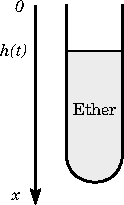
\includegraphics[width=0.3\textwidth]{diffusion_ether.pdf}
\end{figure}

\begin{enumerate}

	\item En notant $c(x)$ la concentration molaire en vapeur d'éther dans le tube entre $0$ et $h(t)$, retrouver l'équation de diffusion sur $c(x)$ en supposant la loi de Fick vérifiée.
	
	\item En déduire la concentration de vapeur d'éther $c(x)$ dans le tube en fonction de $x$, $h(t)$, $P_{sat}$, $R$ et $T$. On supposera qu'on est en régime quasi-stationnaire.
	
	\item Quelle quantité d'éther $dN$ est évaporée entre $t$ et $t+dt$ ? 
	
	\item En déduire l'équation différentielle suivante :
	\begin{align*}
		h\dot{h}=C		
	\end{align*}
	où $C$ est une constante que l'on précisera.
	
	\item En déduire un ordre de grandeur du temps d'évaporation de l'éther.

\end{enumerate}

\newpage

\begin{correction}

\begin{enumerate}

	\item Le grand classique :
	\begin{align*}
		\frac{\partial c}{\partial t}= D\frac{\partial^2 c}{\partial x^2} 
	\end{align*}
	
	\item En RP, $c(x)=Ax+B$. Avec les CL :
	\begin{align*}
		c(x)=\frac{P_{sat}}{RT}\frac{x}{h(t)}
	\end{align*}
	
	\item On a $dN=\frac{\mu}{M}S(h(t+dt)-h(t)$. Mais aussi $dN=-j(x=h(t))S=\frac{P_{sat}}{RT}\frac{D}{h(t)}$
	
	\item On en déduit l'équation :
	\begin{align*}
		h\dot{h}=\frac{DP_{sat}M}{R\mu}		
	\end{align*}
	
	\item En déduire un ordre de grandeur du temps d'évaporation de l'éther.

\end{enumerate}

\end{correction}